\documentclass{article}
\usepackage{fullpage}
\usepackage{graphicx} % Required for inserting images
\usepackage[section]{placeins}
\usepackage{float}
\usepackage{amsmath}
\usepackage{url}
\usepackage{enumitem}

\usepackage{graphicx}
\usepackage{amsmath}
\usepackage{amssymb}
\usepackage{cite}
% \usepackage{flushend} % balance columns after references
\usepackage{booktabs} % table
\usepackage{makecell} % table cell wrapping
\usepackage{enumitem} % nosep
\usepackage{listings}
\usepackage{xcolor}
\usepackage{accsupp}
\usepackage[utf8]{inputenc}
\usepackage{tikz}
\usetikzlibrary{shapes.geometric, arrows.meta, positioning}
\usepackage{pgfplots}

%\usepackage[margin=0.75in]{geometry}
\usepackage{authblk}
\usepackage{url}
\usepackage{algorithm}
\usepackage{algpseudocode}
\algblockdefx[EVENT]{Event}{EndEvent}%
  [1]{\textbf{on event}\ \texttt{#1}\ \algorithmicdo}%
  {\algorithmicend\ \textbf{on}}
\algblockdefx[MESSAGE]{Message}{EndMessage}%
  [2][msg]{\textbf{upon message}\ <\texttt{#1}\ |\ #2>\ \algorithmicdo}%
  {\algorithmicend\ \textbf{upon}}
\algnewcommand{\Assert}{\textbf{assert}\xspace}
\MakeRobust{\Call} % for nested Calls

\newtheorem{definition}{Definition}

\tikzset{
    block/.style={rectangle, draw, text centered, minimum height=2em, minimum width=5cm},
    triangle/.style={regular polygon, regular polygon sides=3, draw, minimum size=3cm},
    arrow/.style={-{Latex}},
    labelstyle/.style={font=\normalsize},
}

\lstset{
    showstringspaces=false,
    basicstyle=\small\ttfamily,
    numbers=none,
    breaklines=true,
    breakatwhitespace=true,
    columns=fullflexible,
    %breakindent=2ex,
    postbreak=\raisebox{0ex}[0ex][0ex]{\BeginAccSupp{ActualText={}}\ensuremath{\color{gray}\hookrightarrow\space}\EndAccSupp{}},
    tabsize=3
}

% ABNF listings
\usepackage[utf8]{inputenc} % Use UTF-8 encoding for modern Unicode handling
\usepackage{listings}
\lstset{
    basicstyle=\ttfamily,
    breaklines=true,
    breakatwhitespace=true,
    tabsize=2,
    columns=fullflexible,
    texcl=true   % tex in listing comments
    escapeinside={\%*}{*)},
    extendedchars=true,
    keepspaces=true,
    showstringspaces=false,
}
\lstdefinelanguage{abnf}{
        comment=[l]{;},
        identifierstyle=\bfseries
}

% \setlength{\parindent}{0pt}
% \setlength{\leftmargin}{1em}
\setlist[itemize]{nosep,itemsep=.1ex}
\setlist[description]{nosep,labelwidth=2em,itemsep=.2ex}
\setlength{\parindent}{0pt}
\setlength{\parskip}{1.5ex}

\setcounter{secnumdepth}{1}

\title{Unicity: Verifiable Off-Chain Agents}
\author{The Unicity Developers\\info@unicity-labs.com}
\date{}

\begin{document}
\maketitle

\begin{abstract}

Unicity is a novel blockchain architecture designed for the development of decentralized applications through a network of off-chain verifiable agents. The primary innovation is to disaggregate the uniqueness (non-forking) proof for the blockchain as a whole, enabling uniqueness proofs to be generated for individual agents executing in parallel off-chain. This approach eliminates two significant scaling bottlenecks of traditional designs: (a)~there is no restriction on size as agents are not stored on-chain, and (b)~there are no computational limitations as agents operate locally within their own environments. Optimal efficiency is achieved by eliminating the need for global ordering, with state shared only amongst economically interested parties. Unicity serves as a decentralized microservices platform, deconstructing decentralized applications into small independent agents that can be developed, deployed and orchestrated without a centralized gatekeeper.

\end{abstract}

\section*{TL;DR}

\begin{itemize}
    \item Unicity agents are encapsulations of verifiably unique code and state e.g. a fungible currency token, an NFT, a smart contract, a game NPC, an AI, or any combination thereof. Agent instances execute off-chain and generate/verify proofs when needed to prove unique state histories.
    \item Layered infrastructure: Proof of Work (PoW) trust anchor, BFT consensus, proof aggregation and agent layers.
    \item PoW Layer: Native platform currency. RandomX ASIC resistant hash function. Exponential moving average difficulty adjustment.
    \item BFT Layer: Block reward winners form a subset of validators that operate a BFT Consensus Layer with one second rounds.
    \item Only single input UTXOs are allowed by consensus rules enabling decomposition of the ledger into compact individual coin sub-ledgers, which can then be efficiently transferred to the Agent Layer.
    \item Proof Aggregation Layer: public permissionless infrastructure, operating an append-only fault tolerant Sparse Merkle Tree (SMT). The SMT receives requests in rounds with each round root hash value anchored in the BFT layer and then subsequently in the PoW layer. ZK succinct proofs of consistency for every insertion batch.
    \item SMT tree is built hierarchically. State transition requests from agents are recorded in the tree with proofs of inclusion and non-deletion providing a proof of uniqueness for agent state histories.
    \item Agent Layer: Acts as a decentralized microservices' platform providing the tools to developers to interface with the Unicity Infrastructure and develop, deploy and orchestrate agents. As execution is local, any programming language or development environment can be used.
\end{itemize}

\section{Introduction}

\subsection{Why Build Decentralized Applications?}

Decentralization is not a goal in itself but a means to achieve specific objectives that may not be feasible or optimal in centralized systems. Bitcoin, for example, uses decentralization as a means to achieve censorship resistance and the elimination of trusted third parties in the transfer of value across the Internet. More generally, decentralized applications can offer enhanced trust, transparency, and user empowerment. They can be designed to be resistant to censorship, manipulation, and single points of failure. They can enable new business models and forms of collaboration that were previously impossible or impractical.

Historically, the technical approaches to decentralization using blockchains have come with very significant trade-offs including performance, scalability, privacy and cost. Blockchains as computers are orders of magnitude more expensive than their conventional counterparts. The inherent need for global ordering (sequential execution of contracts) and globally shared state creates bottlenecks that limit performance and struggles to meet the performance demands of truly global, high-throughput systems.

\begin{figure}[H]
    \centering
    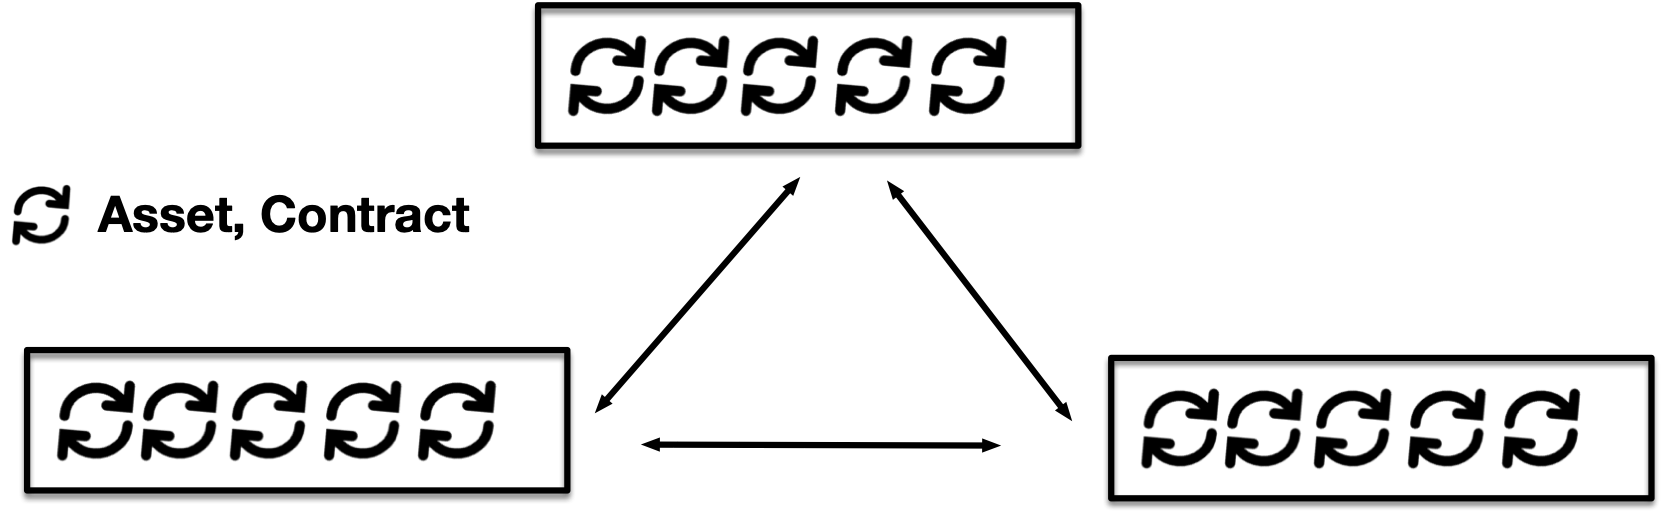
\includegraphics[width=0.6\textwidth]{Legacy.png}
    \caption{Blockchain design}
    \label{fig:legacy}
\end{figure}

The core design principle for blockchains has remained largely the same since the Bitcoin whitepaper was published in 2008. An append-only ledger of assets (and contracts which manipulate those assets) is maintained by a network of nodes with the ledger being updated based on pre-agreed consensus rules. This design inevitably leads to competition for resoures.

\subsection{Programmability}

Bitcoin introduced a basic form of programmability through its scripting language. This limited scripting capability allowed for simple conditions to be attached to transactions, such as multi-signature requirements or time-locked transfers. However, Bitcoin's scripting language was intentionally restricted to maintain the network's security and focus on its primary use case as a digital currency. The concept of a more expansive, programmable blockchain was significantly advanced by Vitalik Buterin with the introduction of Ethereum in 2015. Buterin envisioned a ``world computer''---a global, decentralized platform capable of executing arbitrary code in the form of smart contracts. This vision expanded the blockchain's role from a mere ledger of transactions to a general-purpose computational infrastructure. This progression from Bitcoin's basic scripting to Ethereum's world computer marked a paradigm shift, transforming blockchains from specialized tools for cryptocurrency into general-purpose platforms for decentralized computation and application deployment.

As the complexity and usage of these smart contract platforms have grown, fundamental limitations have become increasingly apparent. Blockchain computers are extremely inefficient with throughput many orders of magnitude lower than a traditional computer. More recent concepts such as alternative consensus protocols, layer-two solutions and sharding introduce various incremental innovations, but these are all workarounds attempting to address the limitations of the original design. For instance, layer-two solutions like rollups for Ethereum can increase transaction throughput by one or two orders of magnitude before they reach a hard limit. They also introduce additional complexity, centralization (centralized sequencers with escape hatches etc.) with potential security vulnerabilities at the points where they interface with the main chain. Sharding is another area of scalability research, however it introduces new challenges in cross-shard communication that can potentially fragment the network's security model. The core issue remains: traditional blockchain architectures struggle to scale without sacrificing either security, decentralization, or both.

\subsection{Unicity: A New Model for Decentralization}

Rather than attempting to optimize within the constraints of traditional blockchain designs, Unicity introduces a fundamentally new approach to building decentralized applications. The core invention is to allow the execution of applications off-chain but with the same cryptographic guarantees as if they were executing on-chain. Assets are minted off-chain, smart contracts are executed off-chain and the blockchain is reduced to an infrastructure that (by enforcement of non-forking) prevents double spending of off-chain assets, each of which is an independent blockchain.

The key cryptographic guarantee that is handled differently in Unicity is proof of uniqueness. Proof of uniqueness, or non-forking, is one of the key proofs that a blockchain provides. In Bitcoin, for example, Proof of Work is used to guarantee that there is a single unique version of the blockchain. The proof of uniqueness in this case is probabilistic, i.e. there may be other copies (forks) but over time the incentive scheme ensures that miners will converge onto the chain with most work (the longest chain rule). This uniqueness proof covers all transactions in a block as all transactions are included in the Proof of Work calculation.

\subsection{The Unicity Architecture}

\begin{figure}[htbp]
    \centering
    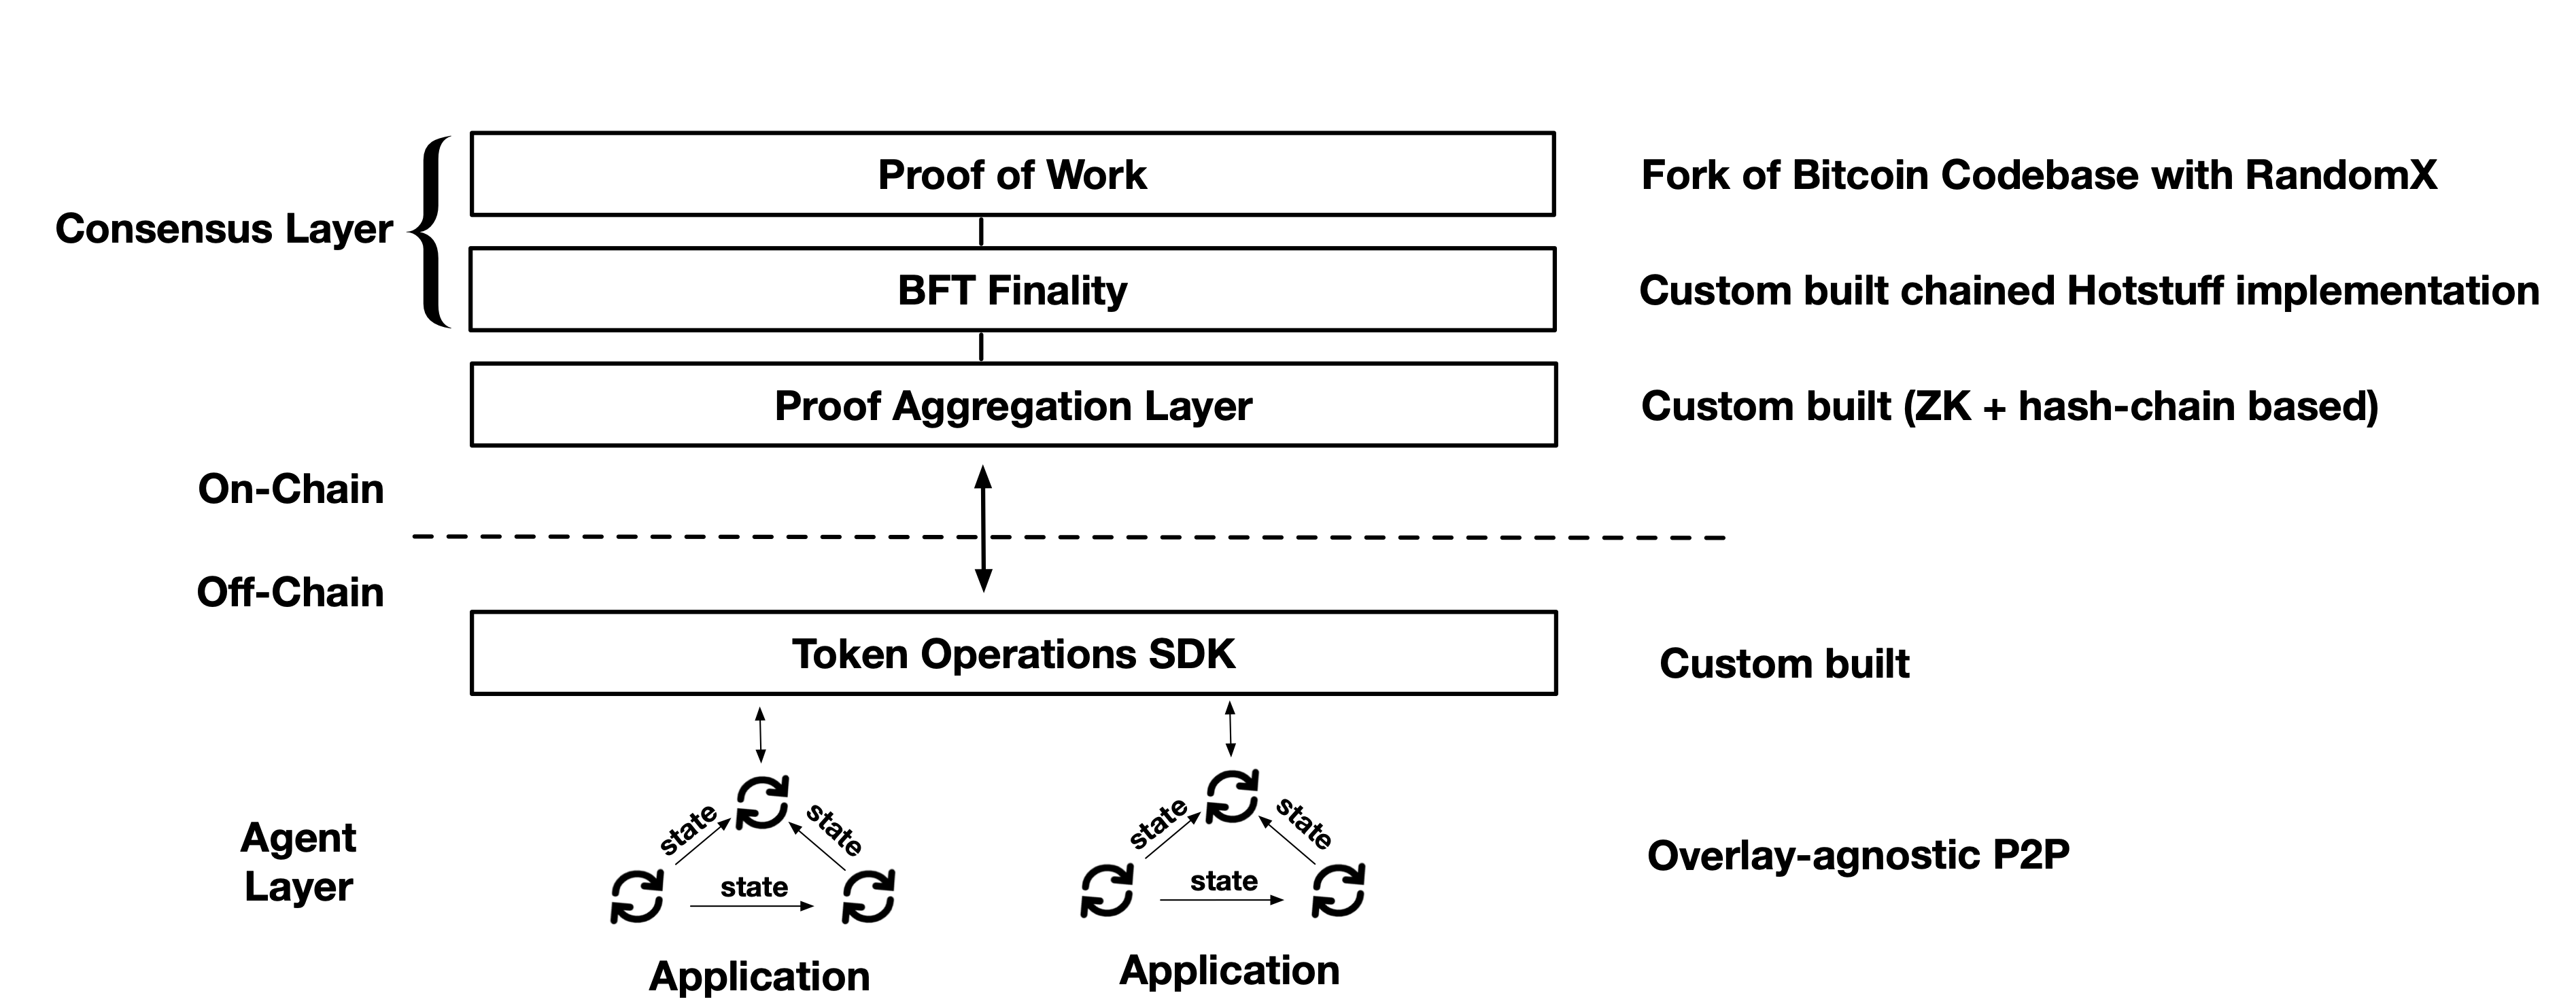
\includegraphics[width=0.8\textwidth]{FullStack.png}
    \caption{Unicity's layered infrastructure}
    \label{fig:layers}
\end{figure}

At an abstract level the Unicity design is divided into three layers. The Consensus layer acts as trust anchor to attest to the uniqueness of local agent state. The public permissionless version of Unicity uses Proof of Work however any Proof system could be used including Proof of Stake, Proof of Authority or trusted hardware. A key point is that the on-chain shared global state is kept to an absolute minimum. Transactions, or more generally \textit{state transitions}, are not included in Consensus Layer blocks.\footnote{Certain transactions may still be necessary. For example, in the Proof of Work implementation coinbase transactions or the distribution of shares in mining pools are still necessary.}
Instead, state transitions happen at the Agent Layer where each agent will order and execute transactions and then send a request to the Proof Aggregation Layer. The requesting agent will receive back a uniqueness proof for the set of transactions that it executed. Effectively, the Proof Aggregation Layer aggregates requests for agents executing in parallel,  commits the aggregate request to the Consensus Layer and returns to each individual agent a proof of uniqueness for that agent's state history.

Agent instances perform local transaction ordering, obtain a uniqueness proof and synchronize state with other agent instances. There is always an ``interested party'' (players in a game, owners of tokens) to ensure verifiability and availability. For example consider a simple turn-based game played by three players. There are only three interested parties. Running this game on-chain either in an L1 or an L2 implies that all the validators  need to execute the game (and all other games) as part of the consensus process. The Unicity approach would be to define the game logic as an agent template with the three players running agent instances. At each turn the player agent instance would update its state, generate a uniqueness proof and synchronize with other agent instances.

A more fundamental example would be digital cash or agents as fungible currency tokens. In this case, for each token there is a single interested party (whoever has ownership of the token). Whenever two parties wish to transact the sender will update ownership of the token to the recipient, generate a Unicity proof and synchronize its state with a new agent instance created by the recipient. At this point the sender is no longer an interested party.

\section{Implementation: Consensus Layer}

The public blockchain is used both as the trust anchor and as the native currency of the system (for compensating network participants and paying of transaction fees). The blockchain is purpose-built for Unicity as a Proof of Work chain similar to Bitcoin with a few modifications.

\begin{figure}[htbp]
    \centering
    \includegraphics[width=0.7\textwidth]{Miners.png}
    \caption{Consensus Layer with Proof of Work trust anchor}
    \label{fig:miners}
\end{figure}

\begin{itemize}
\setlength{\leftmargin}{1em}
 \item It uses the RandomX ASIC-resistant hashing algorithm.
 \item A subset of miners, based on winning past block rewards, self-select to operate a BFT consensus subnet operating at one-second block times. The BFT subnet implements a finality gadget to periodically ensure settlement finality.
 \item Transactions are restricted to single inputs, enabling the overall ledger to be decomposed into compact individual coin sub-ledgers which can be verified with the same trust assumptions as the full chain.  This allows for the coin sub-ledgers can be extracted from the blockchain and used off-chain, such as for paying transaction fees in the Agent Layer.
\end{itemize}

\subsection{ASIC Resistance and Fair Mining}

Nakamoto's vision for Bitcoin was based on achieving censorship resistance through decentralization, with the idea that anyone with a computer could participate in the network's consensus mechanism through mining. However, the rapid evolution of mining technology, particularly the development of ASICs, introduced an unforeseen challenge to this egalitarian ideal. These machines, designed solely for the purpose of mining, quickly outpaced general-purpose computer hardware in terms of hash rate, leading to a concentration of mining power. The resulting centralization not only deviated from Bitcoin's original decentralized ethos but also introduced potential vulnerabilities to the network, such as increased susceptibility to 51\% attacks and reduced geographical distribution of miners.

In our view Proof of Work is unsurpassed as means to build a fault tolerant censorship resistant network. It ties the security of the system to a physical quantity (energy) and with certain limitations coins can be fairly and transparently distributed. There are certainly limitations to Proof of Work such as potential centralization and slow settlement finality, however these limitations can be overcome with modern technologies.

To prevent centralization of mining power new ASIC resistant hash functions have been developed, of which RandomX represents the state of the art, having been battle-tested in Monero, a privacy preserving cryptocurrency, over several years. Unlike Bitcoin's SHA-256 algorithm, RandomX is designed to be ASIC-resistant and CPU-friendly, leveling the playing field and helping maintain a decentralized network of miners. This democratization not only improves network security through wider participation but also upholds the original Bitcoin vision as a decentralized financial system accessible to all. RandomX works by generating random code for each mining round, including a variety of CPU instructions, memory-hard operations and random code execution that can be efficiently performed by general-purpose processors but challenging to optimize in hardware. This ensures that CPUs remain competitive in mining, preserving the network's decentralization and resistance to the concentration of mining power.

\subsection{Ledger Decomposition}

A simple but key innovation in the Consensus Layer is to restrict UTXOs to single inputs.

\begin{minipage}{\linewidth}
\begin{lstlisting}[language=C++]
if (tx.vin.size() != 1)
    return state.Invalid(TxValidationResult::TX_CONSENSUS,
                         "bad-txns-too-many-inputs",
                         "Transactions must have exactly one input");
\end{lstlisting}
\end{minipage}

Due to the restriction on inputs it is possible to extract a compact single coin sub-ledger from the ledger and transfer it to the Agent Layer for programmability, scalability and privacy.

\begin{figure}[H]
    \centering
    \includegraphics[width=0.8\textwidth]{CoinLedger.png}
    \caption{Decomposition into coin sub-ledgers}
    \label{fig:coinledger}
\end{figure}

Coin splits (not shown in the diagram above) are allowed as they don't break the local verifiability, i.e., the verifiability of a single coin depends only on the history of that coin and not the rest of the ledger.

\section{Implementation: Proof Aggregation Layer}

\begin{figure}[htbp]
    \centering
    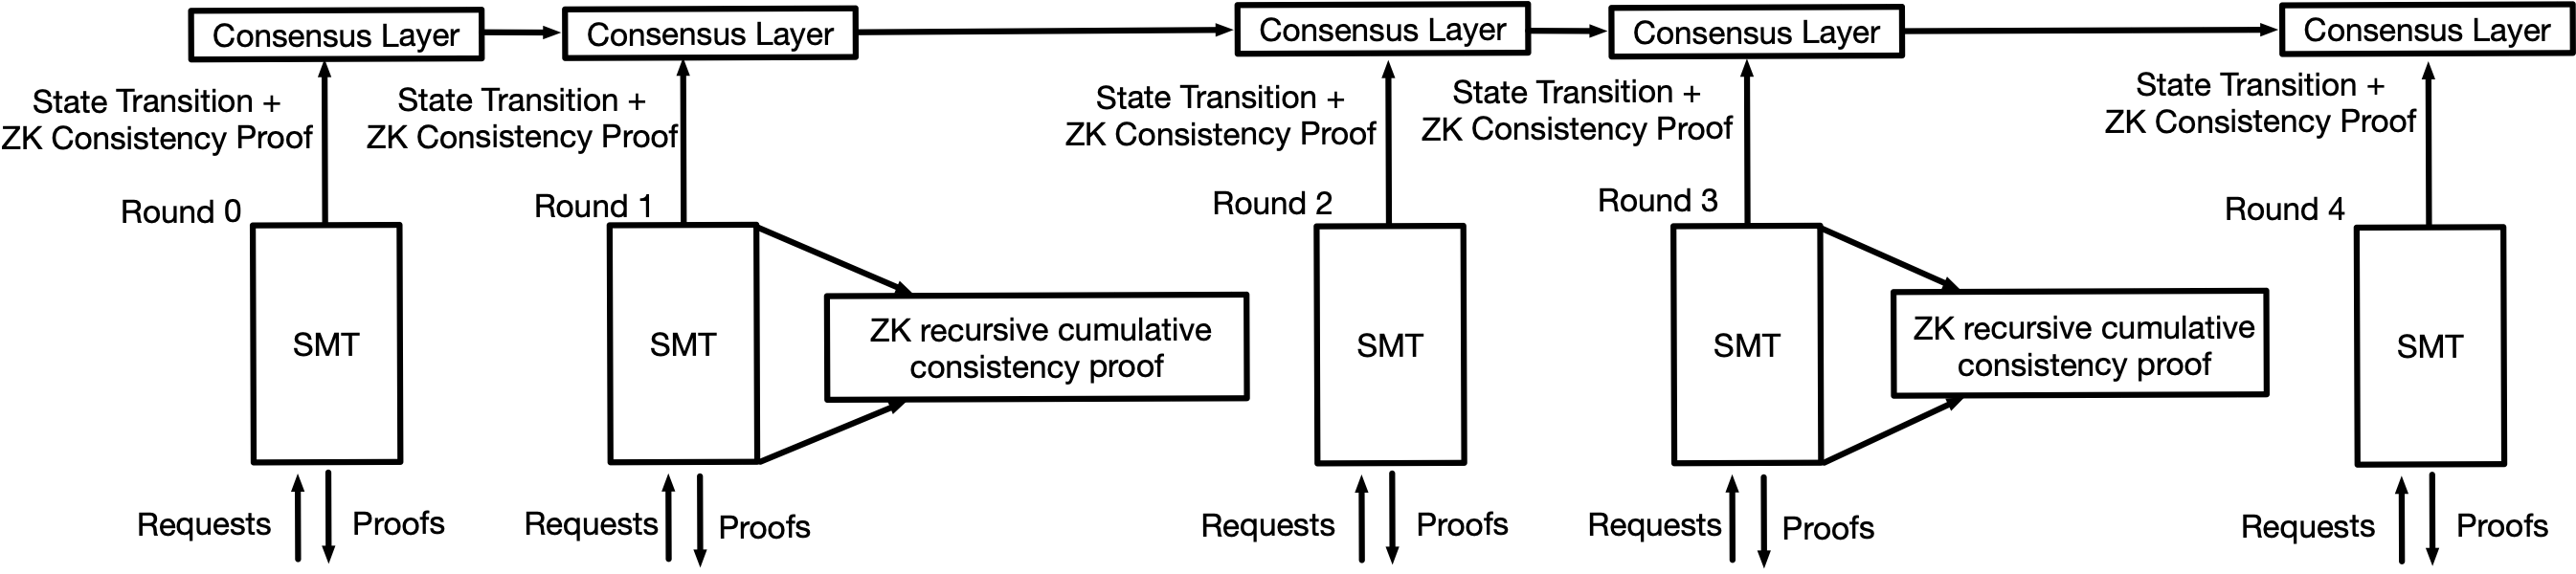
\includegraphics[width=1\textwidth]{SMT-Infra2.png}
    \caption{Proof Aggregation Layer}
    \label{fig:SMT}
\end{figure}

A Sparse Merkle Tree (SMT) is used such that each unique state transition request from the agent layer is allocated a leaf node in the tree. The details of the request will be described in the next section. The SMT is updated in rounds with a batch of state transition requests per round. In each round the SMT state root is calculated, a ZK SMT consistency proof\footnote{The ZK consistency proof proves that no recorded state transitions were modified or removed during the round.} generated and the SMT state transition (previous SMT state root, new SMT state root, ZK SMT consistency proof) is passed to the Consensus Layer. The validators in the Consensus Layer authenticate the request and verify the ZK SMT consistency proof, and then commit to the new SMT root and return a certificate, or cryptographic proof of acceptance of the valid change. After that only requests from the SMT which update the new state root can be accepted.

In a hierarchical trustless system, the principle is that the base layer (e.g., L1 blockchain) provides decentralization, while the layers below it (e.g., rollups) present cryptographic proofs of the correctness of their operation. In scaling Unicity, we have designed efficient data structures to prove the correctness of operation of Aggregation Layer to the Consensus Layer. Based on cryptographic hashes alone, the consistency proof grows linearly with respect to the number of user transactions. This imposes a hard limit of approx. $10\,000$ transactions per second (tx/s), beyond which the networking bandwidth of the Consensus Layer becomes the bottleneck.

To scale further, we must use cryptographic zero-knowledge proofs (ZKPs) to compress the size of the consistency proofs. As an application of ZKPs, this use-case is fundamentally more efficient than using ZKPs to process the transaction data itself, as is done in many privacy coins and ZK-rollups.

$10\,000$ tx/s \emph{per shard} represents the proving throughput achievable on a single consumer-class computer. Due to the small proof size and efficient verification, the Consensus Layer can support a practically unlimited number of such trustless shards. Table~\ref{tab:zk-comparison} compares different ZKP technologies. We have picked subjectively the most appropriate ZK schemes and supporting front-ends (``stacks''). See the bluepaper\footnote{https://github.com/unicitynetwork/aggr-layer-paper/releases/} for full technical details.

\begin{table*}[h!]
    \centering
    \caption{Comparison of zero-knowledge proof technologies for compression of non-deletion proofs}
    \label{tab:zk-comparison}
    \begin{tabular}{@{}lccccccc@{}}
        \toprule
        \textbf{ZK Stack} &
        \makecell{\textbf{Hash}\\\textbf{Function}} &
        \makecell{\textbf{Proving}\\\textbf{Speed (tx/s)}} &
        \makecell{\textbf{Proof}\\\textbf{Size}} &
        \makecell{\textbf{Proof Size}\\\textbf{Asymptotics}} &
        \makecell{\textbf{Trusted}\\\textbf{Setup}} &
        %\makecell{\textbf{PQ}\\\textbf{Secure}} &
        \makecell{\textbf{Impl.}\\\textbf{Effort}} \\
        \midrule
        None (``hash based'') & SHA-256 & 10\,000\textsuperscript{*} & 10\;MB & $O(n)$ & No & N/A \\
        CIRCOM + Groth16         & Poseidon & 25 & 250\;b & $O(1)$ & Yes & Lower \\
        Gnark + Groth16          & Poseidon & 30 & 250\;b & $O(1)$ & Yes & Low \\
        SP1 zkVM  & SHA-256 & 1.5 & 2\;MB & $O(\log n)$ & No & Lowest \\
        Cairo~0 + STwo    & Poseidon2 & 60\textsuperscript{†} & 2.4\;MB & $O(\log n)$ & No & Medium \\
        AIR + Plonky3  & Poseidon2 & 10\,000 & 1.7\;MB & $O(\log n)$ & No & High \\
        AIR + Plonky3   & Poseidon2 & 2500 & 0.7\;MB & $O(\log n)$ & No & High \\
        AIR + Plonky3   & Blake3 & 250 & 1.7\;MB & $O(\log n)$ & No & High \\
        \bottomrule
    \end{tabular}

    \vspace{0.5em}
    \raggedright
    \textsuperscript{*} Bandwidth-limited, no verification effort reduction.\\
    \textsuperscript{†} Trace generation before proving is impractically slow.\\
\end{table*}

The Aggregation Layer is built in a hierarchical manner using smaller size SMT sub-trees. An Aggregator, or machine that operates a sub-tree is algorithmically assigned a place in the overall infrastructure according to network demand. Aggregators are incentivized to join the network based on transaction fees that are shared across the Aggregator pool. The infrastructure is designed to be highly redundant and parallelizable i.e. the tree can be dynamically sub-divided into subtrees which operate asynchronously in parallel with redundancy provided by multiple Aggregators processing the same sub-tree.

\begin{figure}[htbp]
    \centering
    \vspace{\baselineskip}
    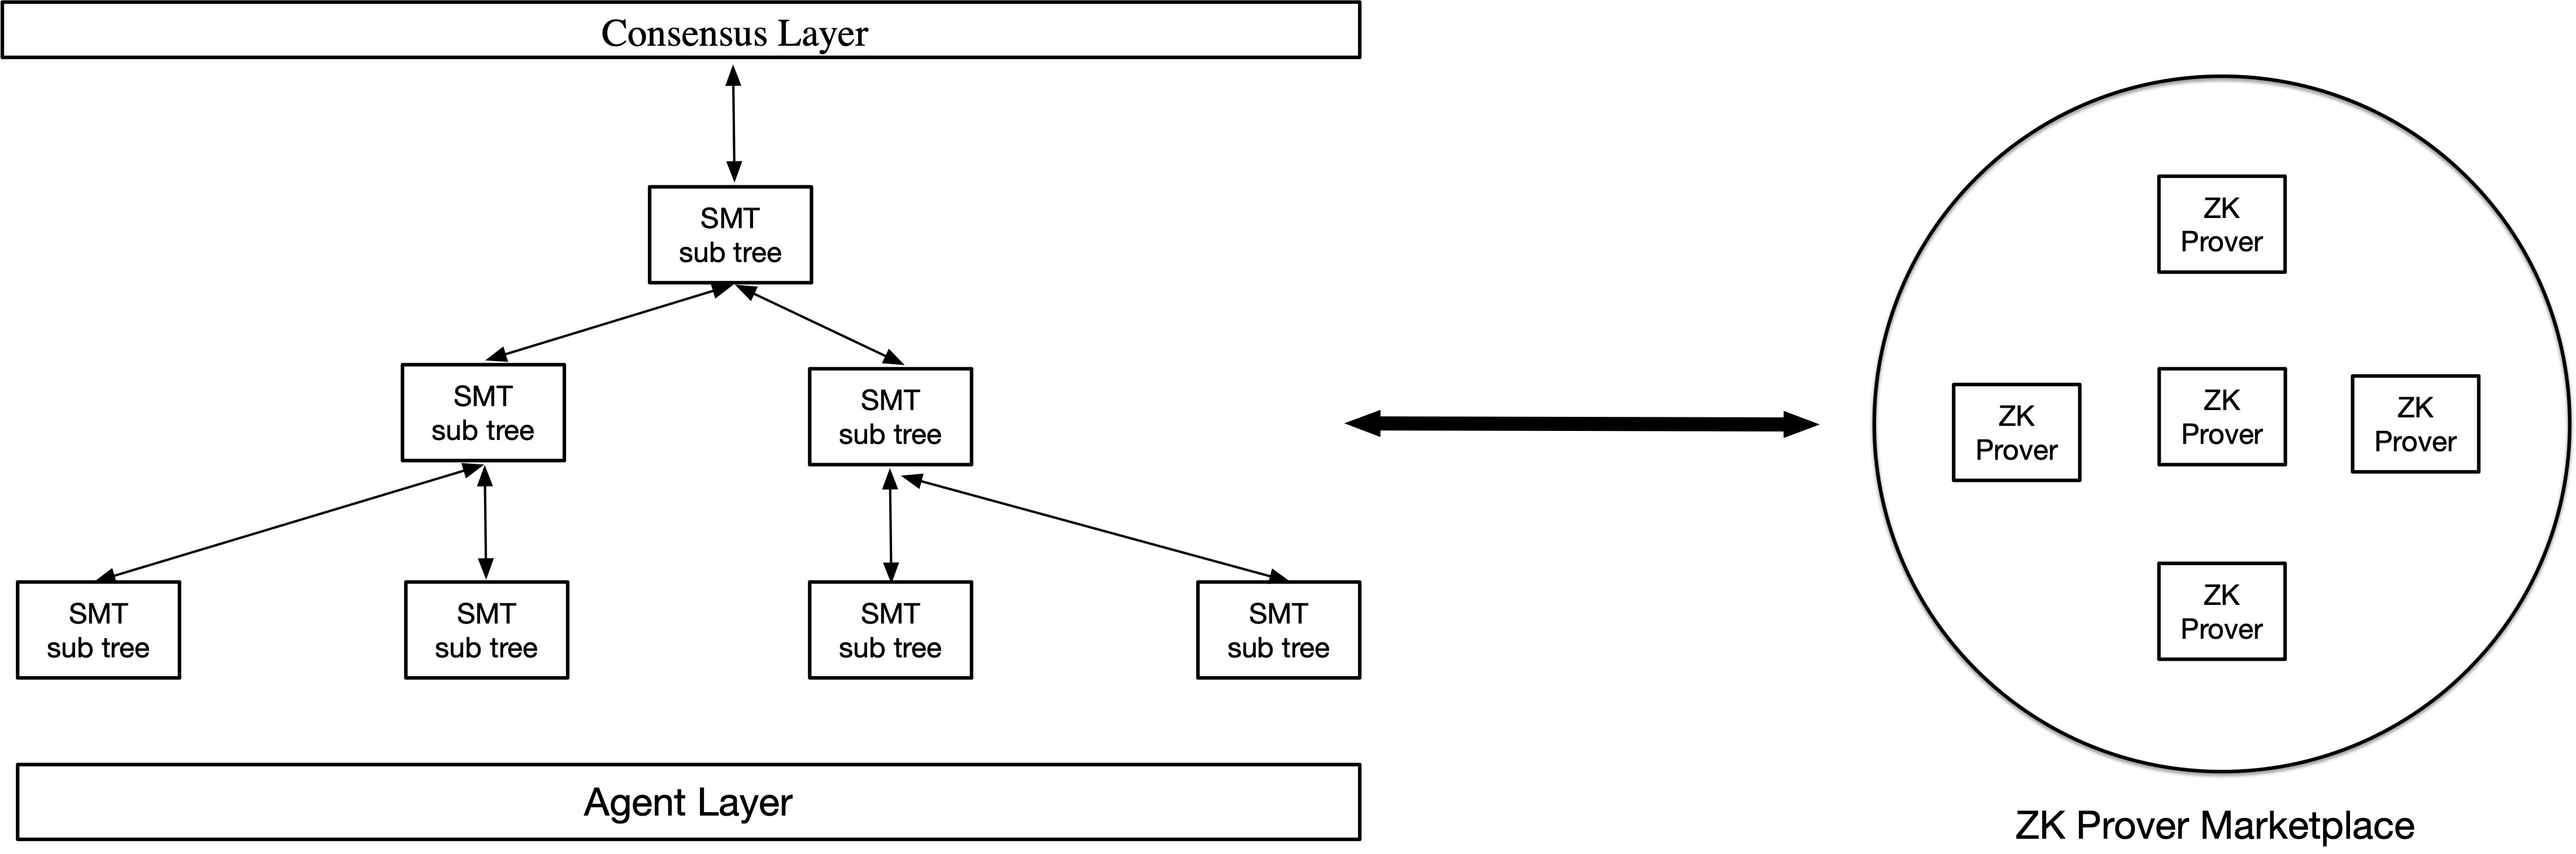
\includegraphics[width=0.7\textwidth]{SMT-ProverMarketPlace.png}
    \caption{Aggregator hierarchical infrastructure}
    \label{fig:SMT-Infra}
\end{figure}

\section{Token Operations}

The Token Operations SDK is a Unicity TypeScript library\footnote{https://github.com/unicitynetwork/state-transition-sdk} that allows the integration of token operations such as minting or transferring into off-chain applications.

A transfer of a token off-chain between a buyer and seller of goods is shown in Figure~\ref{fig:LowLatency1}:

\begin{itemize}
  \item The Buyer creates a commitment\footnote{The unlocking condition for the ownership predicate, such as a digital signature.} that authorizes transfer to the Seller.
  \item The Buyer sends the state transition request to the Unicity infrastructure (Proof Aggregation Layer) which will return an inclusion proof in approximately two seconds. An inclusion proof proves that a state transition is unique i.e., it has happened precisely once.
  \item The Buyer then sends the token + commitment + inclusion proof to the Seller.
  \item The Seller verifies the inclusion proof and releases the goods.\footnote{Note that, for trustless exchange of digital assets, the token transfer and goods release steps can be made atomic using the token predicate system.}
\end{itemize}

\begin{figure}[ht]
    \centering
    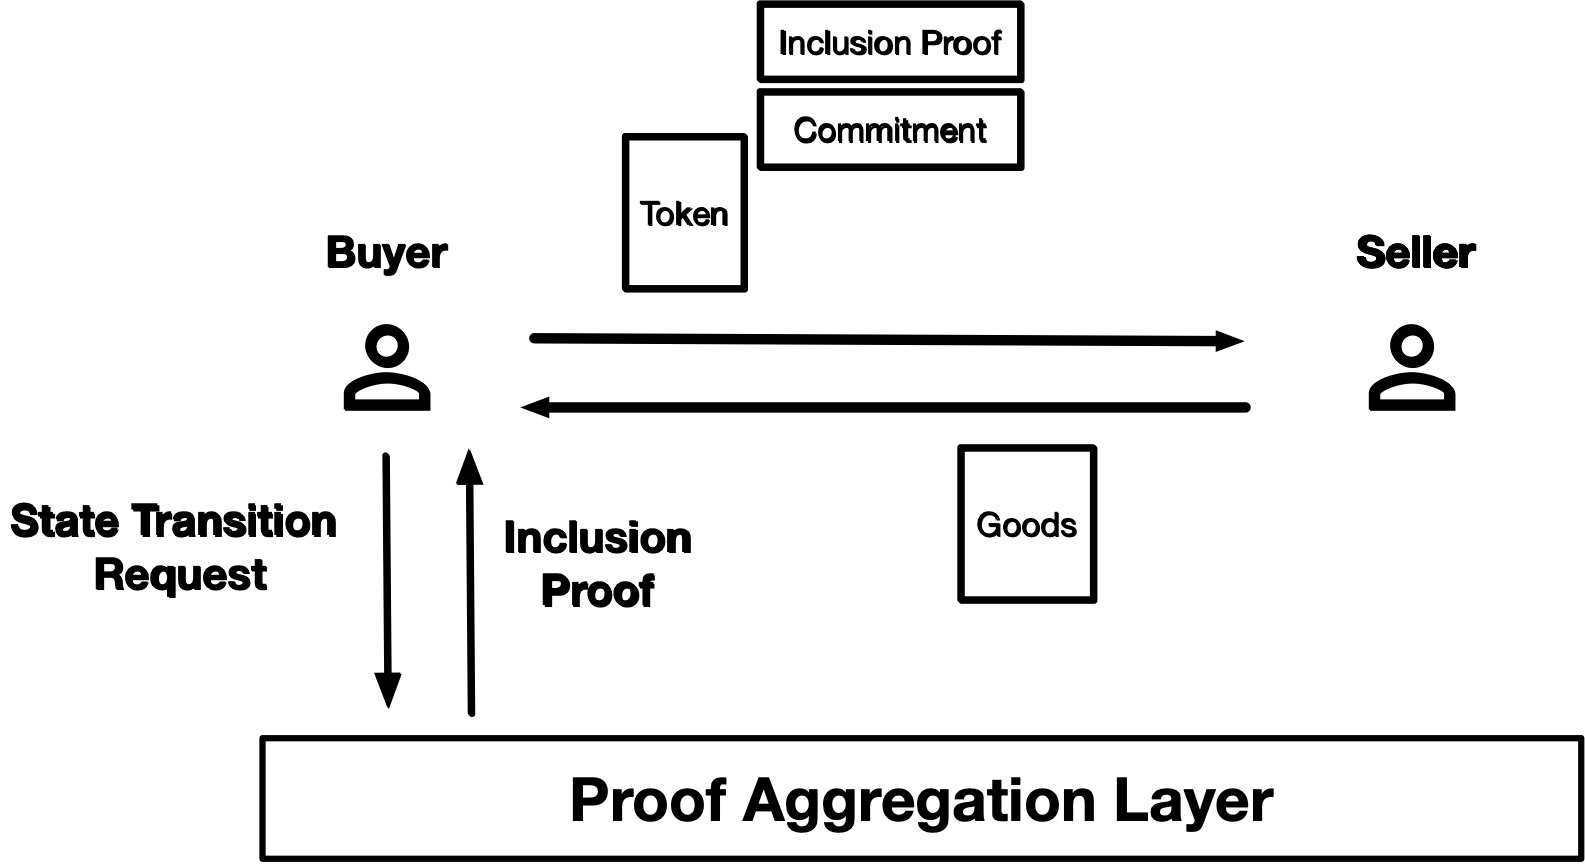
\includegraphics[width=0.6\textwidth]{Transaction1.png}
    \caption{Regular transaction flow with proof of inclusion before the transfer}
    \label{fig:LowLatency1}
\end{figure}

To reduce latency, an extension of the protocol for high frequency trading is as shown on Figure~\ref{fig:LowLatency2}:
\begin{itemize}
  \item The Buyer produces the commitment that authorizes transfer to the Seller.
  \item The Buyer sends the token + commitment to the Seller.
  \item The Seller generates the state transition request, sends it to the Proof Aggregation Layer, and receives back an immediate exclusion proof: a confirmation that this state transition has not been registered before and is now scheduled to be registered.
  \item The Seller releases the goods.
  \item Finally, the Seller waits (approximately two seconds) for the inclusion proof before the received token can be added to usable inventory.
\end{itemize}

Provided that participants have sufficient inventory of tokens for the two second latency, extreme volumes of high frequency transactions can be achieved.

\begin{figure}[ht]
    \centering
    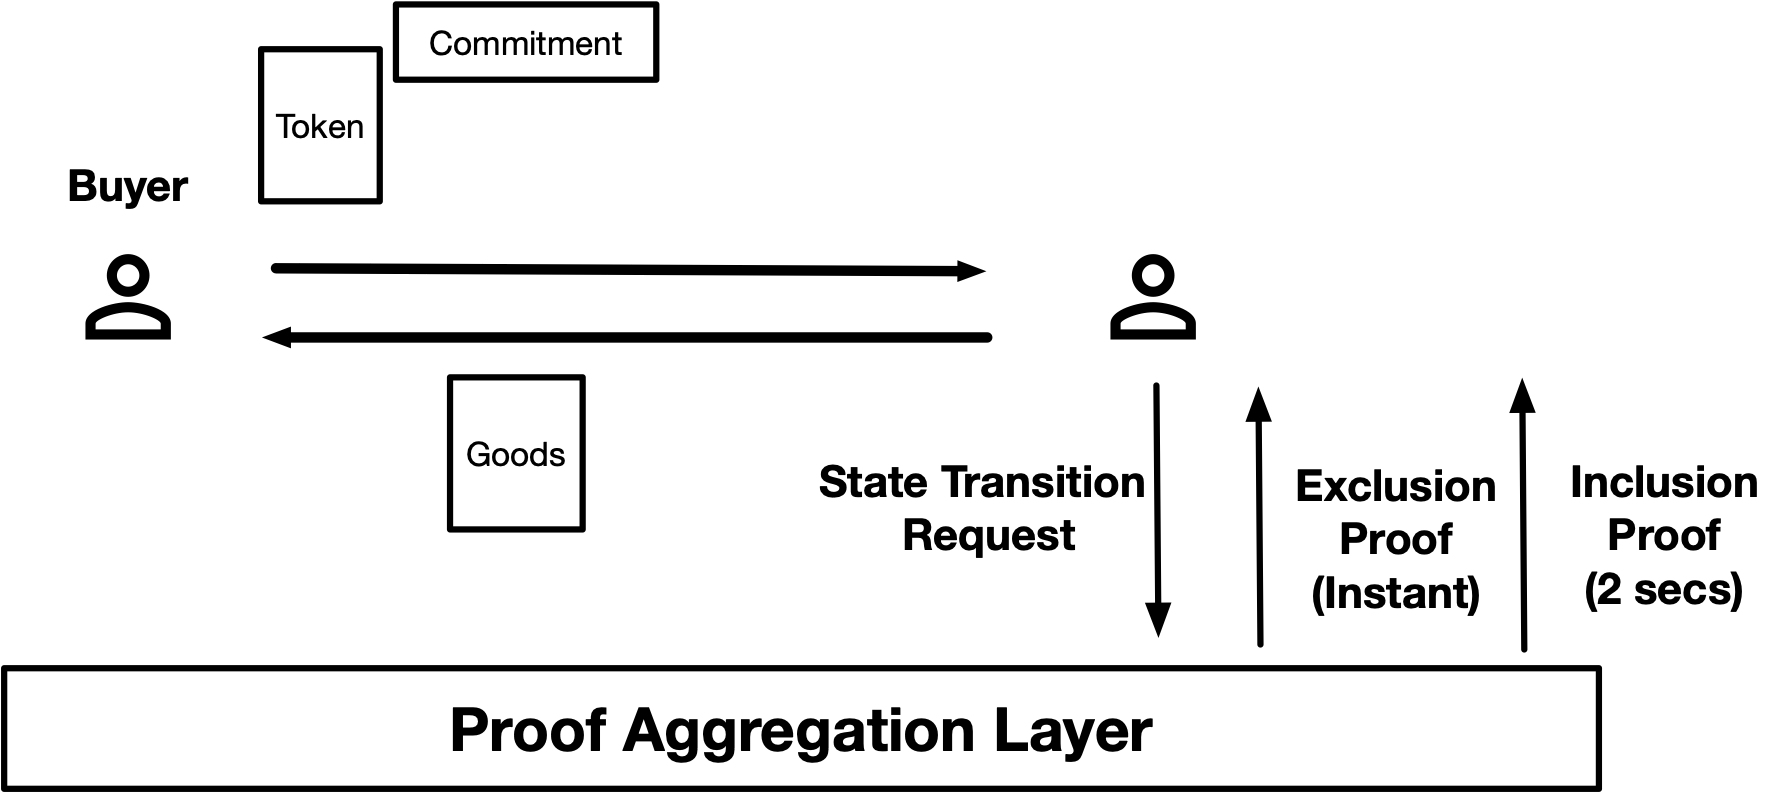
\includegraphics[width=0.6\textwidth]{Transaction2.png}
    \caption{Low-latency transaction flow with proof of inclusion after the transfer}
    \label{fig:LowLatency2}
\end{figure}

\subsection{Off-Line Transactions}

Unicity can support off-line transactions in two distinct ways: assisted by certified secure hardware or using time-locking of tokens designated for off-line spending to predefined recipients.

\paragraph{Zero-trust:}

In this mode, a payer prepares for off-line payments to predefined payees by posting special transfers while still on-line. In those special transfers, the control of each token is set to a conditional ``if the next transition is posted before time~$T$, it must be signed by~$X$; otherwise it must be signed by~$Y$'', where $X$ is the prospective payee and $Y$ is the payer. Then, if the payer decides to make the off-line payment, they can do so by handing a copy of the token's current state over to the payee; the payee can verify that they are indeed the sole controller of the token until time~$T$ and can execute any valid transactions (including taking unconditional ownership of the token) by posting them on-line before time~$T$. If the payer decides to not make the payment, they just have to refrain from making the token's current state available to the payee until time~$T$ when the control of the token reverts to the payer.

\begin{figure}[ht]
    \centering
    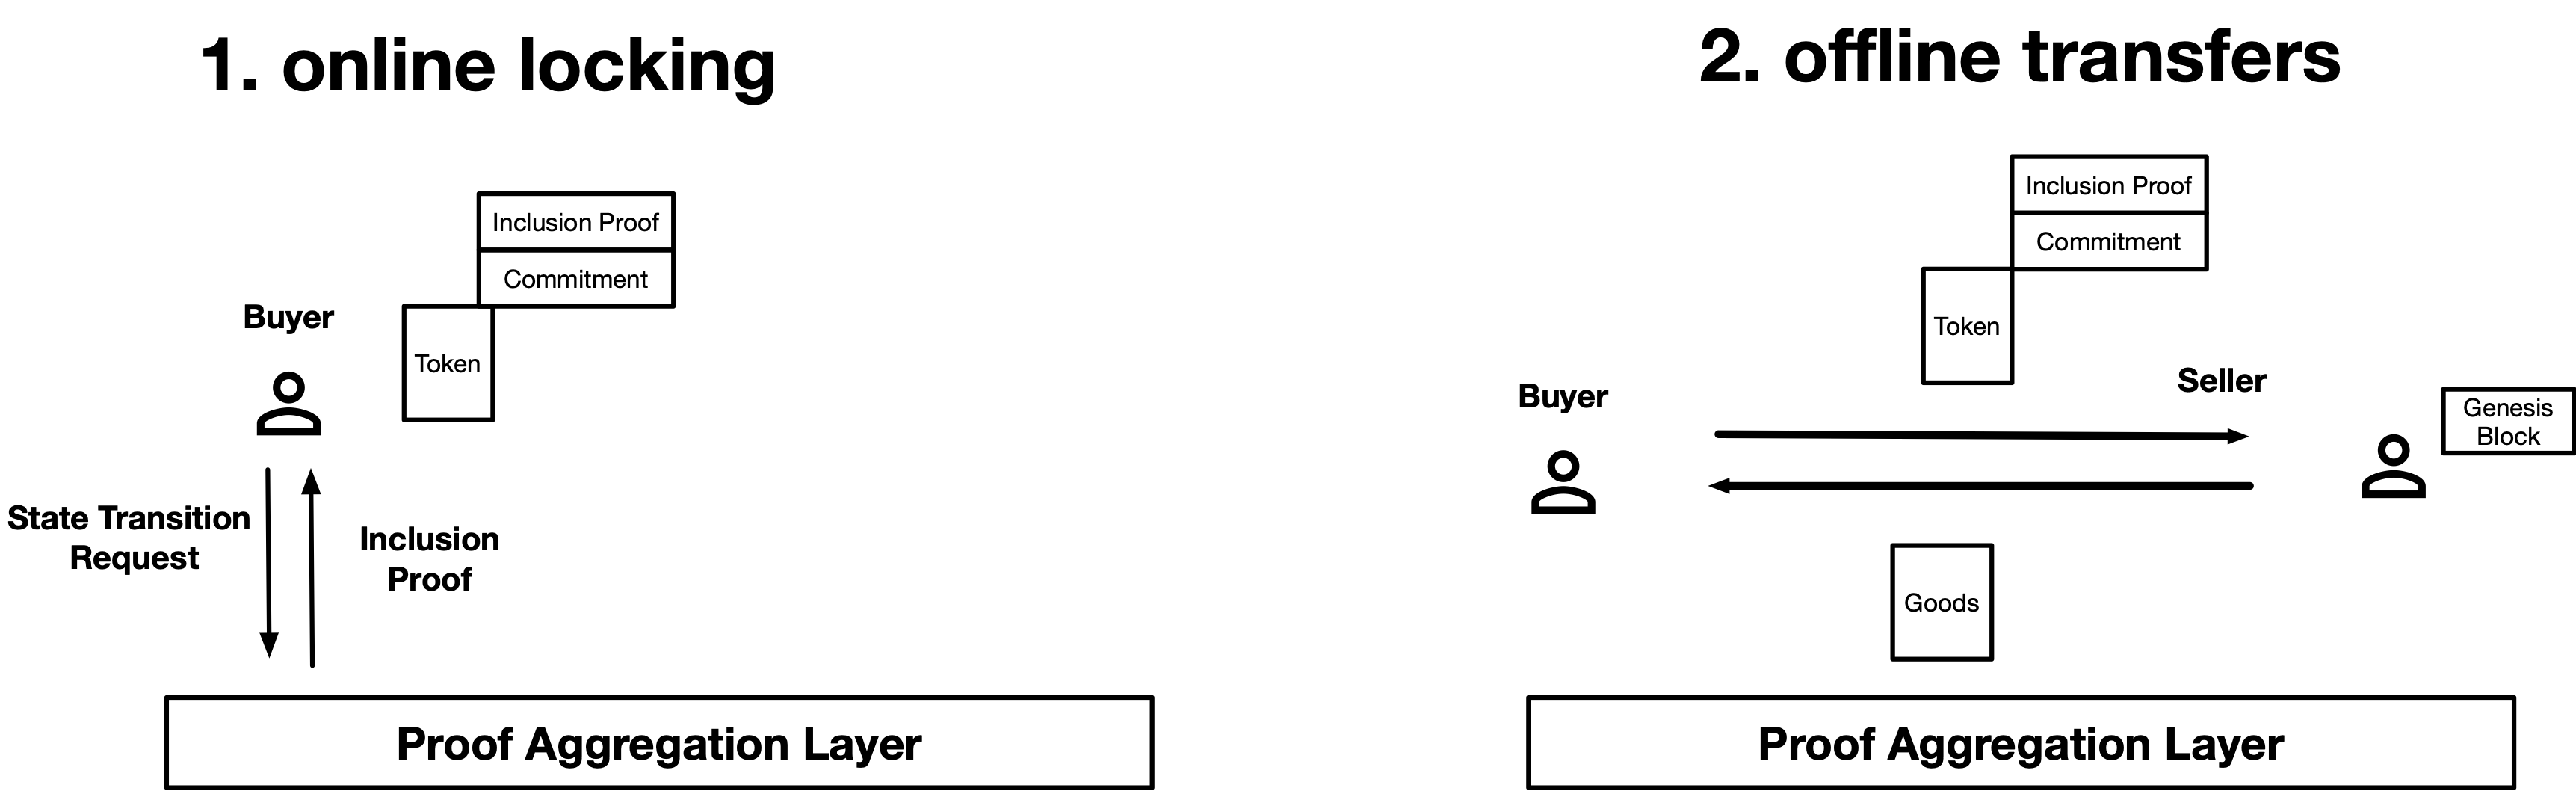
\includegraphics[width=0.9\textwidth]{offline_lock.png}
    \caption{Off-line transactions with zero trust}
    \label{fig:Offline}
\end{figure}

\paragraph{Assisted by secure hardware:}

In this mode, tokens are moved from on-line usage to off-line usage by first executing an on-line transaction transferring the ownership to a certified hardware device. After that, all off-line transfers must be signed by certified devices (and this property must be verified by each subsequent recipient) until the whole chain is eventually posted on-line by the last off-line recipient. Each off-line wallet must be restricted to only sign state transitions where (a)~the wallet is the current owner of the token, and (b)~the wallet has not previously signed any other transition from the same state. With careful implementation, the requirements on the trusted hardware components do not exceed those on the SIM cards of mobile phones. In case one of the devices breaches the protocol, the malfunctioning device can be identified (and appropriate sanctions imposed) when the transition chain is posted on-line.

\subsection{Cross-Chain Transactions}

The network supports minting tokens directly off-chain (e.g. stablecoins) or efficient and secure bridging of tokens minted on external blockchains. Bridged token's genesis record is (1)~ZK proof of external blockchain block header's correctness, (2)~(appropriately locked) token, and (3)~hash chain certifying the token. This information is verified by every subsequent recipient of token transactions.

\begin{figure}[ht]
    \centering
    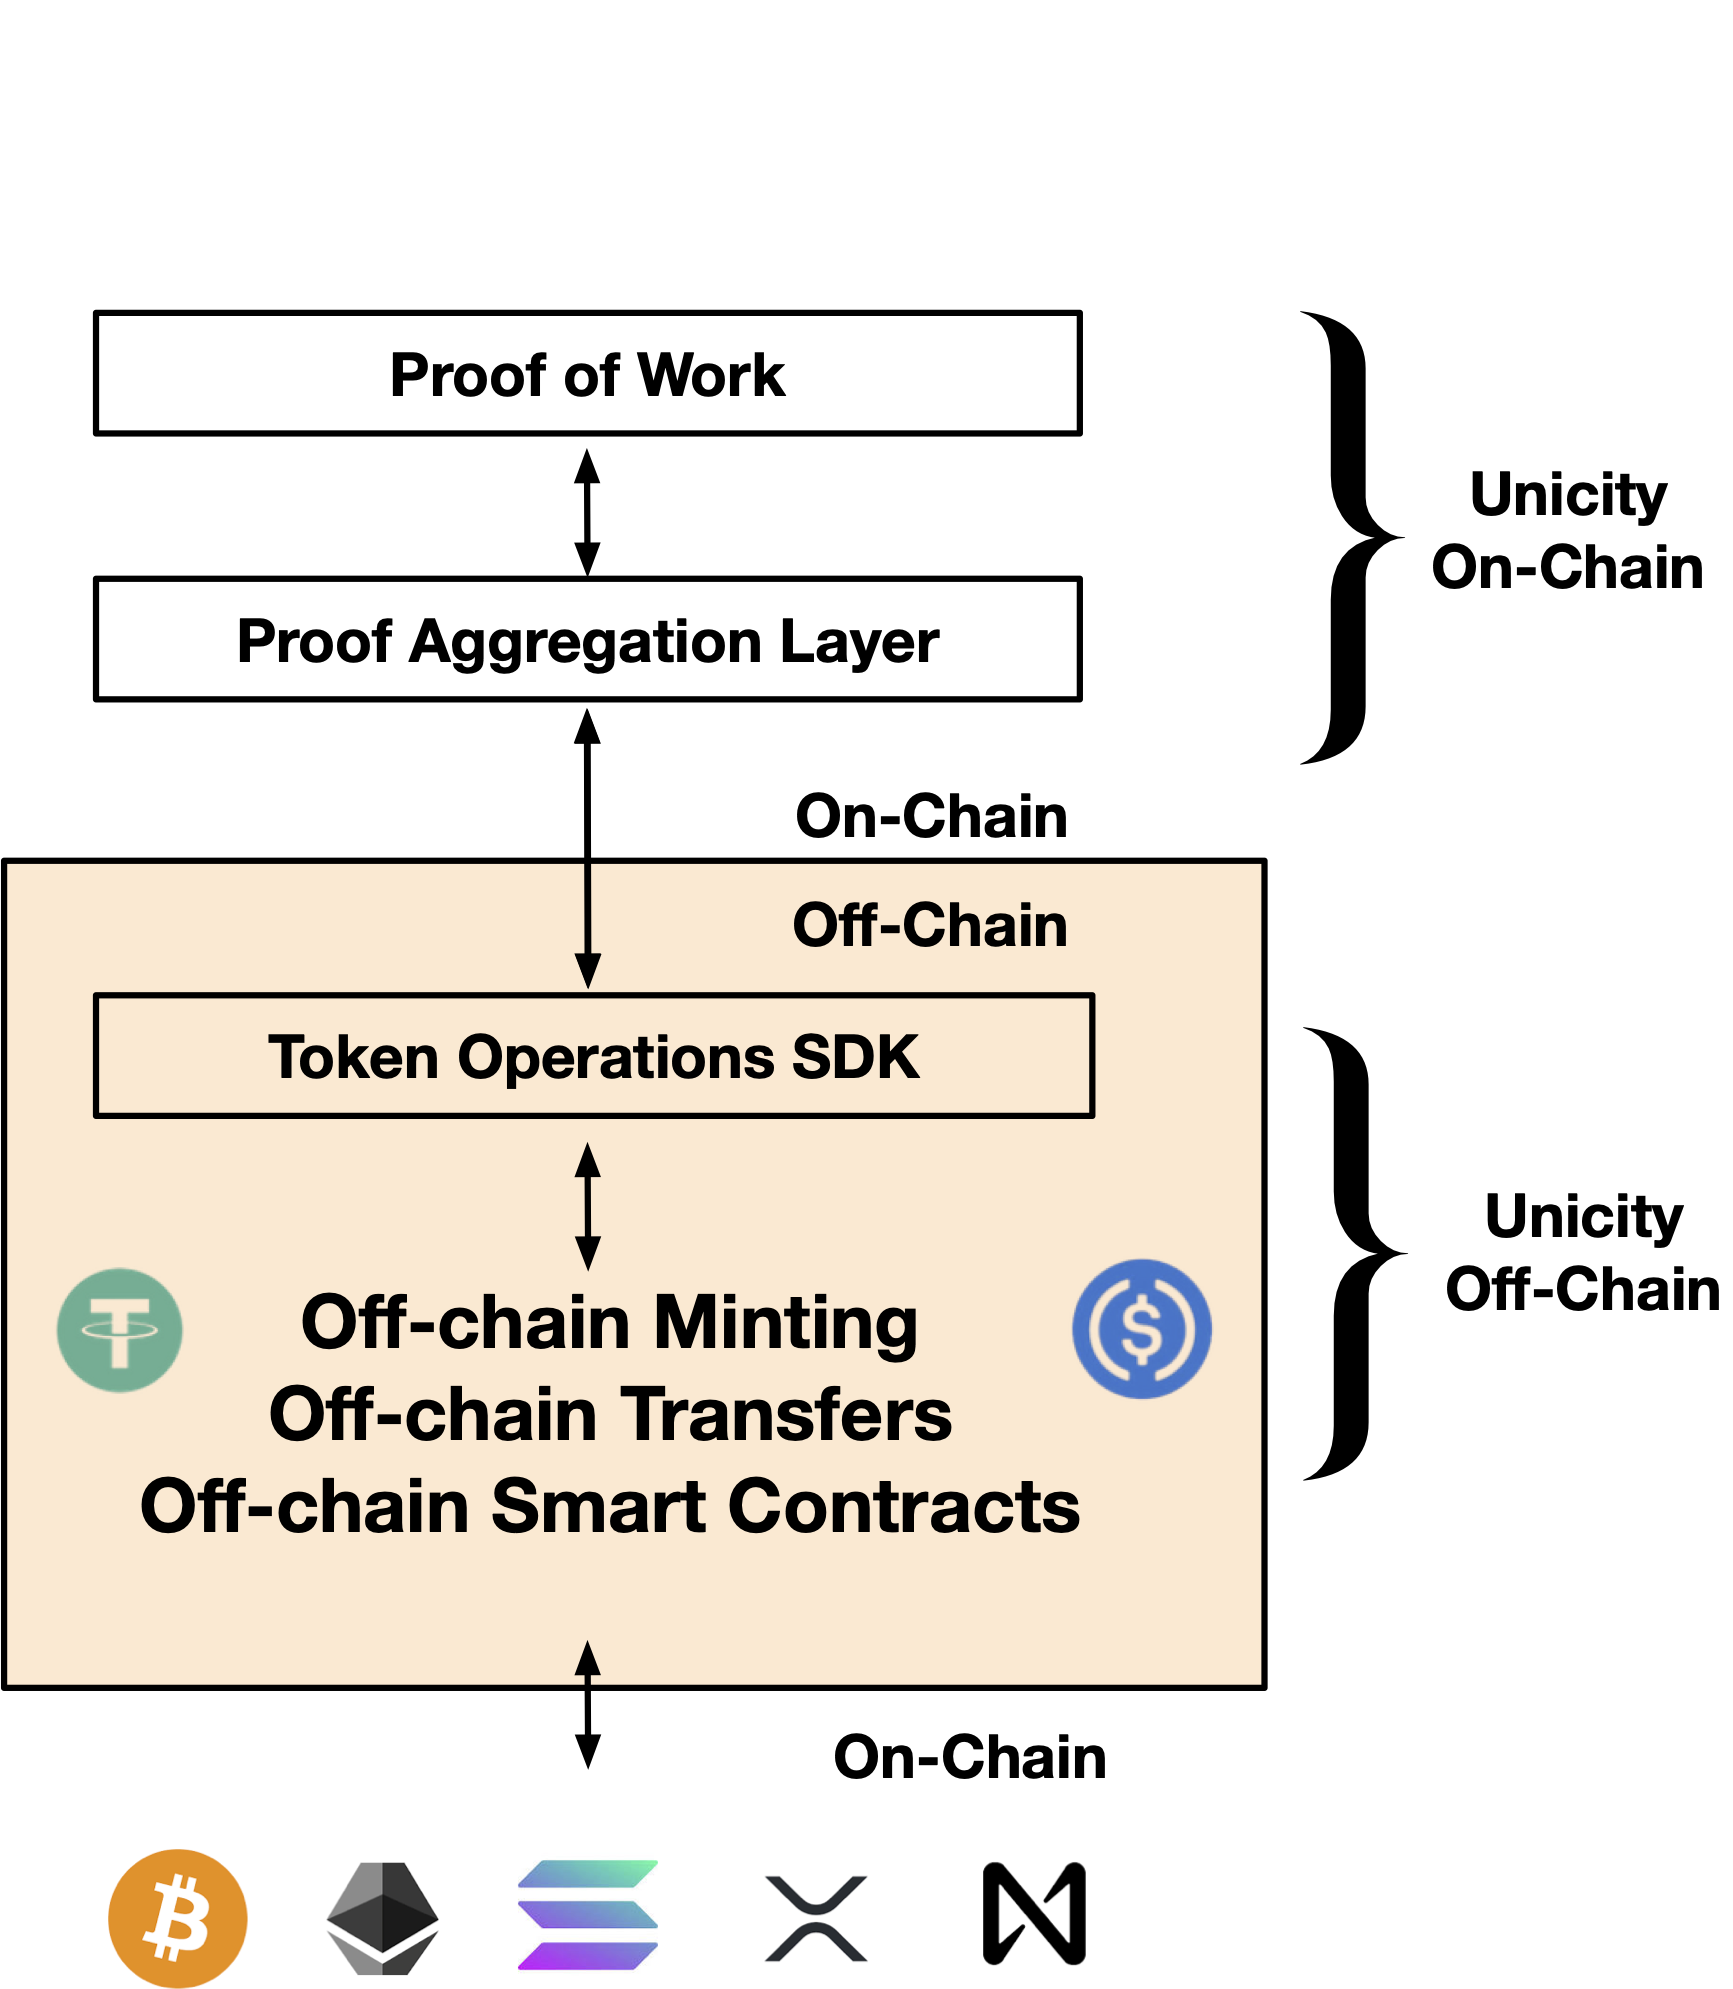
\includegraphics[width=0.5\textwidth]{crosschain.png}
    \caption{Cross-chain transactions}
    \label{fig:CrossChain}
\end{figure}

Bridged tokens are first-class citizens. Token type meta-data and verification code is available to transaction recipients. Elective token history compression by out-of-band ZK prover merges this check into one recursive ZK proof. If the origin blockchain does not support contract verification (e.g. Bitcoin) then a committee-based approach with economic security must be used.

\section{Trust Model}
There are effectively two trust models in Unicity. One is the maximalist zero trust Bitcoin model and the other is a more practical ``trust an honest majority of validators'' seen in today's Proof of Stake chains. The Aggregation Layer is always trustless, as its outputs carry the proof of correct execution and there are no feasible attacks beyond denial of service.

\subsection{Maximalist Trust Model}

In the maximalist model, we assume that users are capable of validating all aspects of system operation that are relevant to their own assets. This level of trustlessness is close to the strong guarantees introduced by Bitcoin, where each ``client'' functions as a full validator, downloading and verifying the blockchain from the genesis block. The Root of Trust is the PoW blockchain. A maximalist user maintains a full node of this chain. Because there are no user transactions, this is relatively lightweight, growing at a few MB a year.

Upon receiving a token, the user must be able to efficiently verify the following:
\begin{enumerate}
    \item The token is valid.
    \item The Aggregation Layer has not forked.
    \item The Aggregation Layer has not certified conflicting states of the same token.
\end{enumerate}

The second point is addressed by validating a unique state root snapshot embedded in the PoW block header. Since the cumulative state snapshot appears with a delay, the block can only be considered final after a snapshot publishing and block confirmation period; hence, maximalist verification is not instantaneous.

The third point is addressed by auditing the operation of the Aggregation Layer, specifically, ensuring that no inclusion proofs have been generated for the token that are not reflected in its recorded history. To achieve this, all non-deletion proofs from the token's genesis up to its current state must be validated. This is made efficient through the use of recursive zero-knowledge proofs (ZKPs), which show that each round's non-deletion proof is valid and that no rounds were skipped from verification. These recursive proofs are generated periodically and are made available with some latency.

\subsection{Practical Trust Model}

If we relax the model by assuming that a majority of BFT consensus nodes exhibit economically rational behavior and do not collude maliciously with the Aggregation Layer, the user can enjoy significantly more practical operational parameters. BFT layer forking (case 2 above) or certifying conflicting states (case 3 above) produces strong cryptographic evidence (enables slashing and other after-the-fact measures) which is processed out of the critical path of serving users.

In this scenario, a transaction is finalized, and an inclusion proof is returned within a few seconds, allowing the transaction to be immediately verified by independent, non-connected parties.

\section{Implementation: Agent Layer}

The Agent Layer is used to build decentralized censorship resistant applications in Unicity. Each application may consist of multiple agents (e.g. trading pair CLOBs, game NPCs etc). This replicates the functionality of on-chain smart contracts in traditional blockchains, with the obvious difference that the execution is local and running off-chain in parallel. The Agent SDK provides tools for agent development, agent to agent communication and interfacing with the Unicity infrastructure for proof generation.

\begin{figure}[ht]
    \centering
    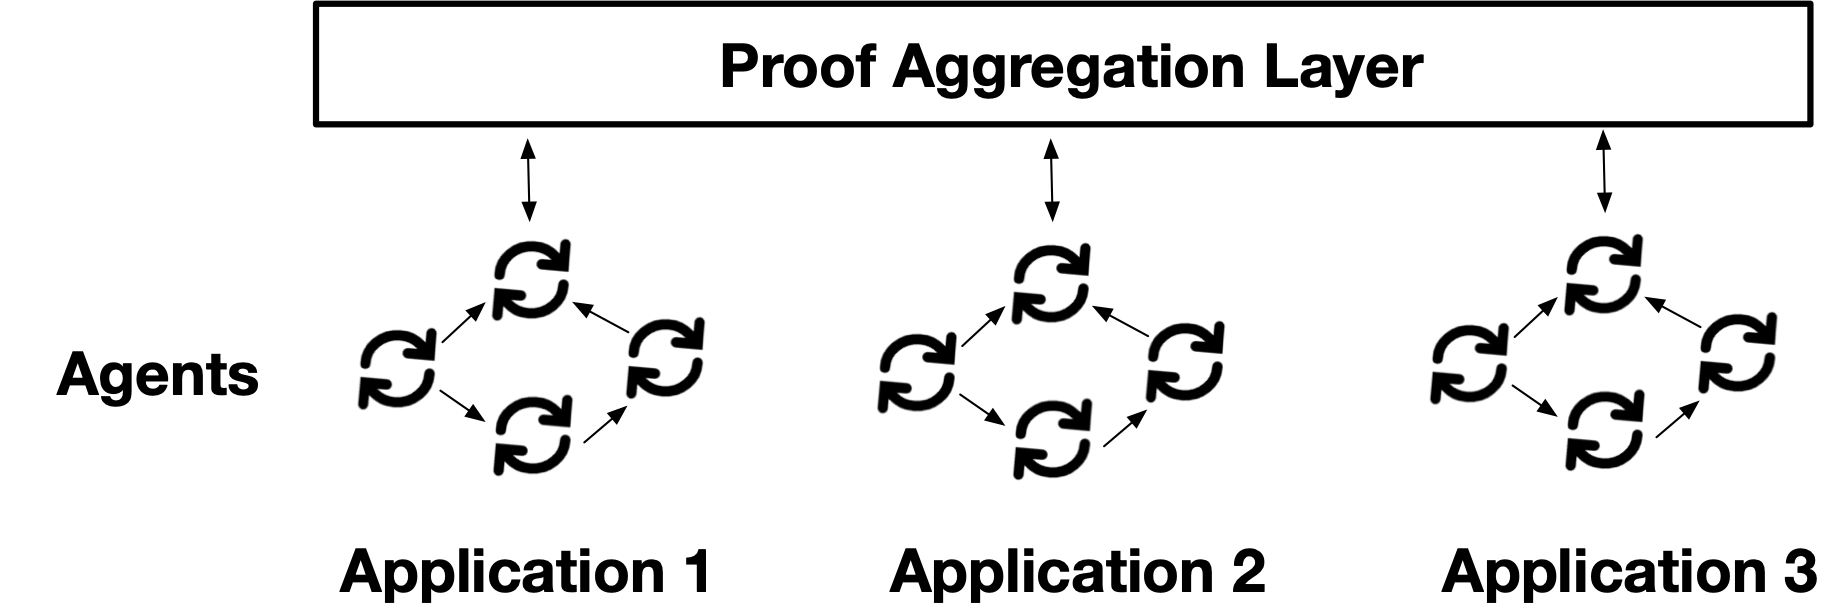
\includegraphics[width=0.6\textwidth]{AgentContracts.png}
    \caption{Unicity agents}
    \label{fig:AgentContracts}
\end{figure}

Agents can be composed for building on-line applications with familiar Web2 development experience and performance while possessing Web3 security properties (decentralization, censorship-resistance, verifiability). A critical point is that settlement is local i.e. agents do not depend on the state of other agents to execute. All agents are independent and execute locally in their own environments without referring to the state of other agents. This is in contrast to smart contract platforms such as Ethereum in which smart contracts have full access to other smart contracts' state, as all code and state exists within the memory of a single instance of the Ethereum Virtual Machine.

Agents are agnostic to the execution environment i.e. they can run on backend, frontend, as stand-alone apps, as parts of some other application, process, etc., with communication/storage infrastructure depending on the application's requirements.

Agents are also agnostic to transport/communication and data sharing channels (direct TCP/IP, UDP, WebRTC, cloud-based shared documents, app-based instant messaging, etc).

Agents can be non-deterministic (though verifiable), and can be written in any language and tech stack.

Agent instances are self-authenticated and universally addressable (no matter where and how an agent instance is running, it can be addressed and connected to by its unique self-authenticated identifer).

Agents manage their verifiable execution state snapshots within Unicity token state transition framework and exchange verifiable state with other agents---state changes are registered in the Proof Aggregation Layer and can then be verified by other agents.

\subsection{Analogy with Kubernetes: an Agent Approach to Application Deployments}

The Unicity model is a radical departure from traditional blockchain design, allowing massive scale parallelization of agents which interact to execute a decentralized application. An analogy with microservices and Kubernetes is relevant. A microservices architecture involves breaking down an application into small, independent services that can be developed, deployed, and scaled independently, with Kubernetes providing the platform for management and orchestration. The Unicity platform involves breaking down a decentralized application into small independent agents that can be developed, deployed and scaled without a centralized gatekeeper.

\section{Trade-Offs}

As there is no shared global state there are no globally synchronized state-dependent operations such as flash loans or MEV.

Unlike traditional blockchains, there is no public global ledger of asset ownership and unless additional steps are taken the ownership history of a token cannot be traced.  For regulated financial markets it is necessary to introduce additional proofs into the token history for KYC/AML procedures, ensuring compliant transfers at each step.

Traditional blockchains rely on users trusting a validator set who verify computation on the user's behalf. In a client-side model, the user verifies incoming transactions. This approach enhances privacy and censorship resistance by eliminating reliance on third-party validators for direct transaction validation. The client's core task is the deterministic verification of these network-anchored proofs and the token's internal consistency, a focused process designed for security and efficiency.

\section{Decentralized Finance}

There are two compelling reasons for decentralized finance (DeFi). For individuals, the appeal is freedom---the elimination of intermediaries, allowing direct engagement in financial transactions without relying on centralized entities such as banks or payment processors. This provides greater financial autonomy and protection against authoritarian government censorship, ensuring the freedom to transact and access financial services without external control or intervention. For institutions, incorporating elements of DeFi can enhance security and automation by eliminating the need for human oversight. Processes can be streamlined, operational costs reduced, and risks associated with human error or fraud mitigated, while enforcing regulatory compliance at the code level. Whilst these are two very different perspectives, it is clear that DeFi has the potential to revolutionize financial services, driving innovation and empowerment at both the individual and institutional levels.

\begin{figure}[H]
    \centering
    \includegraphics[width=0.7\textwidth]{ABEX.png}
    \caption{Agent-based decentralized exchange}
    \label{fig:ABEX}
\end{figure}

Figure \ref{fig:ABEX} shows a simplistic view of a decentralized exchange built using a set of interacting agents. The core agents are the Central Limit Order Book (CLOB) agents which manage individual trading pairs. Depending on requirements these can be deployed and replicated on consumer laptops for a fully permissionless censorship resistant network, or operating in high-powered servers in high availability data centers. From a functional perspective, the end result is the same. Individual agents execute in parallel, and synchronize state in a fully transparent, verifiable, and autonomous way. Other agents provide KYC access, margin management, act as price oracles and provide any other functionality that is required to operate the exchange.

\section{Decentralized Gaming}

Although blockchain technology has been proposed as a means of enhancing transparency and facilitating value exchange in gaming, its current application has largely been limited to asset tokenization within centralized game architectures. Due to the limitations of existing designs, using blockchain for actual game execution remains impractical. However, the potential benefits of decentralized gaming are clear: players can gain true ownership of interoperable assets across different games, enjoy transparency and community-driven governance, experience censorship resistance, unlock innovative business models like play-to-earn, and support fair reward systems for creators.

The motivation behind this work came from a desire to solve a real problem in the gaming industry. The industry has, to a large degree, converged on a client-server approach and while the accepted view is that although pure client-side execution of multi-player games is technically possible, it considered impractical due to issues of security and synchronization. However, the client-server approach is itself severely limited as it is technically challenging to have many players interact in real-time on the same server instance. Modern simulations are limited to a few hundred players interacting in the same shared world due to this limitation.

Unicity is an attempt to overcome these limitations and build a truly decentralized game engine for massive online multi-player immersive simulations. In this case decentralization is not a ``nice to have'' but an essential requirement to allow complex multi-player interactions with potentially millions of players all interacting online. Moving execution to the client side would allow the system to scale, with blockchain technology providing a security layer that guarantees honest gameplay.

A user will initialize the game environment and interact with a set of agents that execute the game mechanics such as NPCs, real-world assets and in-game assets. As users interact with the virtual world and approach other players, the players' agents will synchronize with each other with verifiable state transitions proving that the game logic has been followed and enabling game synchronization and exchange of assets.

\begin{figure}[H]
    \centering
    \includegraphics[width=0.4\textwidth]{game.png}
    \caption{Three-player simulation}
    \label{fig:game}
\end{figure}

In the event of a failed verification action can be taken defined by the game logic, such as rewinding the game to the previous known good state. In this way, a completely new type of game engine can be built with the game components consisting of either autonomous agents, managing game logic, and semi-autonomous agents operating on behalf of the player, and interacting with the environment and other players.

\section{Decentralized AI}

The pace of AI advancement in recent years has been nothing short of breathtaking. From the remarkable performance of Large Language Models (LLMs) to AI systems capable of complex problem-solving and creative tasks, the capabilities of artificial intelligence are expanding exponentially. This rapid progress, while promising to accelerate further, also raises significant concerns about potential risks and unintended consequences of unchecked AI development. As AI systems become more sophisticated and autonomous, there is an urgent need to implement robust guardrails to ensure these powerful technologies remain aligned with human values and societal well-being. However, a world increasingly reliant on AI's probabilistic and often unexplainable models, as opposed to deterministic processes, makes it extremely challenging to implement these guardrails and verify alignment with society's goals and values.

Blockchain technology has been proposed as a means to build transparent and immutable AI systems. However, due to the limited processing power, high latency, and costly nature of on-chain operations, it is impractical to execute complex AI models directly on-chain. The size of AI models far exceeds the storage capabilities of most blockchain platforms, and the slow transaction speeds along with high costs make real-time AI decision-making virtually impossible in a purely on-chain environment. Unicity overcomes these obstacles to the convergence of AI and blockchain technology. Execution happens at native speed off-chain in AI agents' local environments but with the same security guarantees as if agents were executing on-chain. The platform enables the building of verifiable AI systems that allow human operators and agents to interact through trustless state verification, deterministically verifying that execution has been carried out in accordance with agreed rules, and taking action when they do not.

\begin{figure}[H]
    \centering
    \includegraphics[width=0.5\textwidth]{AI.png}
    \caption{Agents coordinating on a task through trustless state verification }
    \label{fig:ai}
\end{figure}

When combined with a native currency as a means to reward agents based on their performance, contributions, or desired behavior, Unicity lays the foundations for a fully secure and verifiable decentralized ecosystem. AI agents can be programmed to earn digital currency for completing tasks, solving problems, or contributing computational resources. This currency acts as the medium of exchange in an agent economy, driving collaboration and competition among AI agents, motivating them to optimize their actions for efficiency and productivity.

The incentive structure  enables the creation of decentralized marketplaces where AI agents can exchange data, services, or computational power with other agents or human participants. Digital currency provides a transparent, automated way to measure the value of contributions, ensuring that autonomous AI systems remain aligned with predefined goals and facilitating verifiability between agents, human operators, and stakeholders. The structure promotes self-sustaining, scalable systems where AI agents evolve and improve autonomously while being rewarded for their beneficial outputs. By addressing the challenges of on-chain AI execution and providing a framework for verifiable, incentivized AI agents, Unicity paves the way for a new era of decentralized artificial intelligence that balances innovation with accountability and alignment with human values.

\end{document}
